% =====================================================================
%  The Evolution of a C-- Compiler
%  This write-up grows together with the source tree.
%    v1  (10 Sep 2026) : Part I  - the lexical analyzer
%    v2  (05 Oct 2026) : Part II - the parser
% =====================================================================
\documentclass[11pt]{article}

\usepackage[T1]{fontenc}
\usepackage{lmodern}
\usepackage[a4paper,margin=1in]{geometry}
\usepackage{amsmath,amssymb}
\usepackage{booktabs}
\usepackage{array}
\usepackage{listings}
\usepackage{xcolor}
\usepackage{tikz}
\usetikzlibrary{automata,positioning,arrows.meta}
\usepackage{hyperref}

\definecolor{codegray}{gray}{0.96}
\lstset{
  basicstyle=\ttfamily\small,
  backgroundcolor=\color{codegray},
  frame=single,
  framerule=0pt,
  breaklines=true,
  columns=fullflexible,
  keepspaces=true,
  showstringspaces=false,
  language=C++,
}

\title{The Evolution of a C-- Compiler\\[0.35em]
       \large Part I --- The Lexical Analyzer}
\author{Abdullah Shoaib\\ \small 23L-0569}
\date{10 September 2026}

\begin{document}
\maketitle

\begin{abstract}
This report follows the construction of a compiler front end for
\textsf{C--}, a small subset of C++. Part~I covers the lexical analyzer: the token classes, the regular definitions of the complex
tokens, a transition diagram that recognizes every token of the language,
and the notes that go with the implementation.
\end{abstract}

\tableofcontents

% =====================================================================
\section{Introduction}
% =====================================================================
\textsf{C--} is a deliberately small language. It supports only two data
types, \texttt{int} and \texttt{char}; there are no arrays and no strings.
The constructs it does support are

\begin{itemize}
  \item declarations (\texttt{int x;}, \texttt{char c = 'a';}),
  \item expressions and store statements,
  \item selection with \texttt{if}--\texttt{else},
  \item iteration with \texttt{while},
  \item functions (definitions, parameters and calls).
\end{itemize}

\noindent
Relational operators are part of the language; logical operators
(\texttt{\&\&}, \texttt{||}, \texttt{!} as a unary operator) are not.
Two special keywords, \texttt{in} and \texttt{out}, are used for input and
output. The work is split into two stages:

\begin{description}
  \item[Lexer] the lexical analyzer (this part),
  \item[Parser] a recursive-descent parser that reuses the lexer.
\end{description}

% =====================================================================
\section{Lexical Analysis}
% =====================================================================

\subsection{Token classes}
Every lexeme produced by the scanner belongs to one of the classes below.

\begin{center}
\begin{tabular}{@{}lll@{}}
\toprule
\textbf{Class} & \textbf{Token type} & \textbf{Examples}\\
\midrule
Identifier            & \texttt{ID}            & \texttt{x}, \texttt{total}, \texttt{factorial}\\
Keyword               & \texttt{KEYWORD}       & \texttt{int}, \texttt{if}, \texttt{while}, \texttt{in}, \texttt{out}\\
Integer literal       & \texttt{INTEGER}       & \texttt{0}, \texttt{42}, \texttt{1000}\\
Character literal     & \texttt{CHAR}          & \texttt{'a'}, \texttt{'Z'}, \texttt{'0'}\\
Arithmetic operator   & \texttt{ARITHMETIC\_OP} & \texttt{+}, \texttt{-}, \texttt{*}, \texttt{/}\\
Relational operator   & \texttt{LT/LTE/GT/GTE/EQ/NEQ} & \texttt{<}, \texttt{<=}, \texttt{>}, \texttt{>=}, \texttt{==}, \texttt{!=}\\
\texttt{=} operator   & \texttt{ASSIGNMENT\_OP} & \texttt{=}\\
Delimiter             & \texttt{DELIMITER}     & \texttt{(} \texttt{)} \texttt{\{} \texttt{\}} \texttt{;} \texttt{,}\\
End of file           & \texttt{EOF}           & ---\\
Error                 & \texttt{ERROR}         & an illegal character\\
\bottomrule
\end{tabular}
\end{center}

\subsection{Regular definitions}
The tokens that have more than one lexeme are described by the following
regular definitions, where \texttt{digit} and \texttt{letter} are the usual
character classes.

\begin{center}
\begin{tabular}{@{}rcl@{}}
\toprule
\textbf{Name} & $\rightarrow$ & \textbf{Regular definition}\\
\midrule
\texttt{digit}    & $\rightarrow$ & \texttt{[0-9]}\\
\texttt{letter}   & $\rightarrow$ & \texttt{[A-Za-z]}\\
\texttt{under}    & $\rightarrow$ & \texttt{\_}\\
\texttt{id}       & $\rightarrow$ & \texttt{letter (letter | digit | under)*}\\
\texttt{integer}  & $\rightarrow$ & \texttt{digit digit*}\\
\texttt{charlit}  & $\rightarrow$ & \texttt{' (any char except ' and newline) '}\\
\texttt{relop}    & $\rightarrow$ & \texttt{< | <= | > | >= | == | !=}\\
\texttt{addop}    & $\rightarrow$ & \texttt{+ | -}\\
\texttt{mulop}    & $\rightarrow$ & \texttt{* | /}\\
\bottomrule
\end{tabular}
\end{center}

\noindent
A lexeme matched by \texttt{id} is looked up in a reserved-word set; if it is
found it becomes a \texttt{KEYWORD}, otherwise it stays an \texttt{ID}. The
two-character relational operators (\texttt{<=}, \texttt{>=}, \texttt{==},
\texttt{!=}) are the reason the scanner needs one character of lookahead.

\subsection{Transition diagram}
Figure~\ref{fig:dfa} is the transition diagram of the scanner. State $q_0$ is
the start state; a state drawn with a double circle is an accepting state and
is labelled with the token class it emits.

\begin{figure}[htbp]
\centering
\resizebox{\textwidth}{!}{%
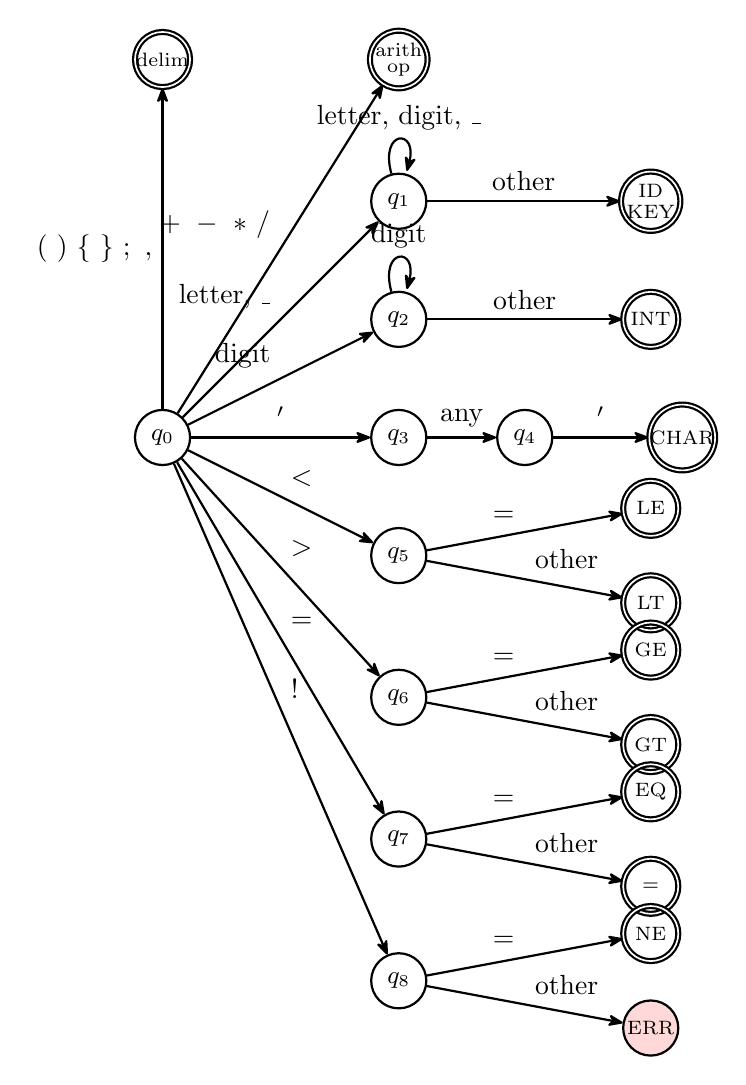
\begin{tikzpicture}[>={Stealth[round]}, auto, thick,
  state/.style={circle, draw, minimum size=7mm, inner sep=0pt, font=\small},
  acc/.style={circle, draw, double, minimum size=7mm, inner sep=0pt, font=\scriptsize},
  err/.style={circle, draw, minimum size=7mm, inner sep=0pt, font=\scriptsize, fill=red!15}]

\node[state] (q0) at (0,0) {$q_0$};

% identifiers / keywords
\node[state] (q1) at (3.0,3.0) {$q_1$};
\node[acc]   (a1) at (6.2,3.0) {\shortstack{ID\\KEY}};
\draw[->] (q0) -- node{letter, \_} (q1);
\draw[->] (q1) edge [loop above] node{letter, digit, \_} (q1);
\draw[->] (q1) -- node{other} (a1);

% integers
\node[state] (q2) at (3.0,1.5) {$q_2$};
\node[acc]   (a2) at (6.2,1.5) {INT};
\draw[->] (q0) -- node{digit} (q2);
\draw[->] (q2) edge [loop above] node{digit} (q2);
\draw[->] (q2) -- node{other} (a2);

% character literals
\node[state] (q3) at (3.0,0.0) {$q_3$};
\node[state] (q4) at (4.6,0.0) {$q_4$};
\node[acc]   (a3) at (6.6,0.0) {CHAR};
\draw[->] (q0) -- node{$\mathrm{'}$} (q3);
\draw[->] (q3) -- node{any} (q4);
\draw[->] (q4) -- node{$\mathrm{'}$} (a3);

% < and <=
\node[state] (ql) at (3.0,-1.5) {$q_5$};
\node[acc]   (alt) at (6.2,-2.1) {LT};
\node[acc]   (ale) at (6.2,-0.9) {LE};
\draw[->] (q0) -- node{$<$} (ql);
\draw[->] (ql) -- node{$=$} (ale);
\draw[->] (ql) -- node{other} (alt);

% > and >=
\node[state] (qg) at (3.0,-3.3) {$q_6$};
\node[acc]   (agt) at (6.2,-3.9) {GT};
\node[acc]   (age) at (6.2,-2.7) {GE};
\draw[->] (q0) -- node{$>$} (qg);
\draw[->] (qg) -- node{$=$} (age);
\draw[->] (qg) -- node{other} (agt);

% = and ==
\node[state] (qe) at (3.0,-5.1) {$q_7$};
\node[acc]   (aas) at (6.2,-5.7) {=};
\node[acc]   (aeq) at (6.2,-4.5) {EQ};
\draw[->] (q0) -- node{$=$} (qe);
\draw[->] (qe) -- node{$=$} (aeq);
\draw[->] (qe) -- node{other} (aas);

% ! and !=
\node[state] (qb) at (3.0,-6.9) {$q_8$};
\node[err]   (aer) at (6.2,-7.5) {ERR};
\node[acc]   (ane) at (6.2,-6.3) {NE};
\draw[->] (q0) -- node{$!$} (qb);
\draw[->] (qb) -- node{$=$} (ane);
\draw[->] (qb) -- node{other} (aer);

% single character accepts
\node[acc] (aop) at (3.0,4.8) {\shortstack{arith\\op}};
\node[acc] (ade) at (0,4.8) {delim};
\draw[->] (q0) -- node{$+\ -\ *\ /$} (aop);
\draw[->] (q0) -- node{$(\ )\ \{\ \}\ ;\ ,$} (ade);

\end{tikzpicture}}
\caption{Transition diagram recognizing every token of \textsf{C--}.
Whitespace is consumed between tokens and is not shown.}
\label{fig:dfa}
\end{figure}

\subsection{Implementation notes}
The scanner is the \texttt{Lexer} class. It keeps the source text together
with a position, a line and a column so that diagnostics can point at the
offending location. Whitespace is skipped before each token, and the public
interface is simply

\begin{lstlisting}
bool hasMoreTokens();
Token nextToken();
\end{lstlisting}

A \texttt{Token} carries its type, its lexeme and the line/column where it
starts. The interesting methods are the ones for the multi-lexeme tokens:
\texttt{scanID} (which also classifies keywords), \texttt{scanInteger} and
\texttt{scanChar}. The scanner reports two lexical errors directly: an
unknown character and a stray \texttt{!} that is not followed by \texttt{=}.

% =====================================================================
\section{Status and next steps}
% =====================================================================
The lexical analyzer is complete: it turns a \textsf{C--} source file into a
stream of typed tokens and reports lexical errors with their position.
The next stage builds the parser on top of this token stream, starting
from a context-free grammar for \textsf{C--} and turning it into a
recursive-descent recognizer.

\end{document}
